% Capitulo 1 - 3.3 Analise e complexidade do algoritmo (MANUSCRITO)
% Tres subcapitulos: um paragrafo direto, o big O e a figura do caderno.
% Para trocar cada espaco reservado pela foto, salve a foto por cima do
% arquivo correspondente em Imagens/Insertion Sort/ mantendo o nome.

\subsubsection{Melhor caso}

\indent \qquad O melhor caso ocorre quando o vetor já está em ordem crescente.
A cada passagem, a primeira comparação do laço interno falha e nenhum elemento é
deslocado: o algoritmo faz $n - 1$ comparações e nada mais. O custo é linear,
$O(n)$. A dedução está na Figura \ref{fig:melhor_caso}.

\begin{figure}[H]
	\centering
	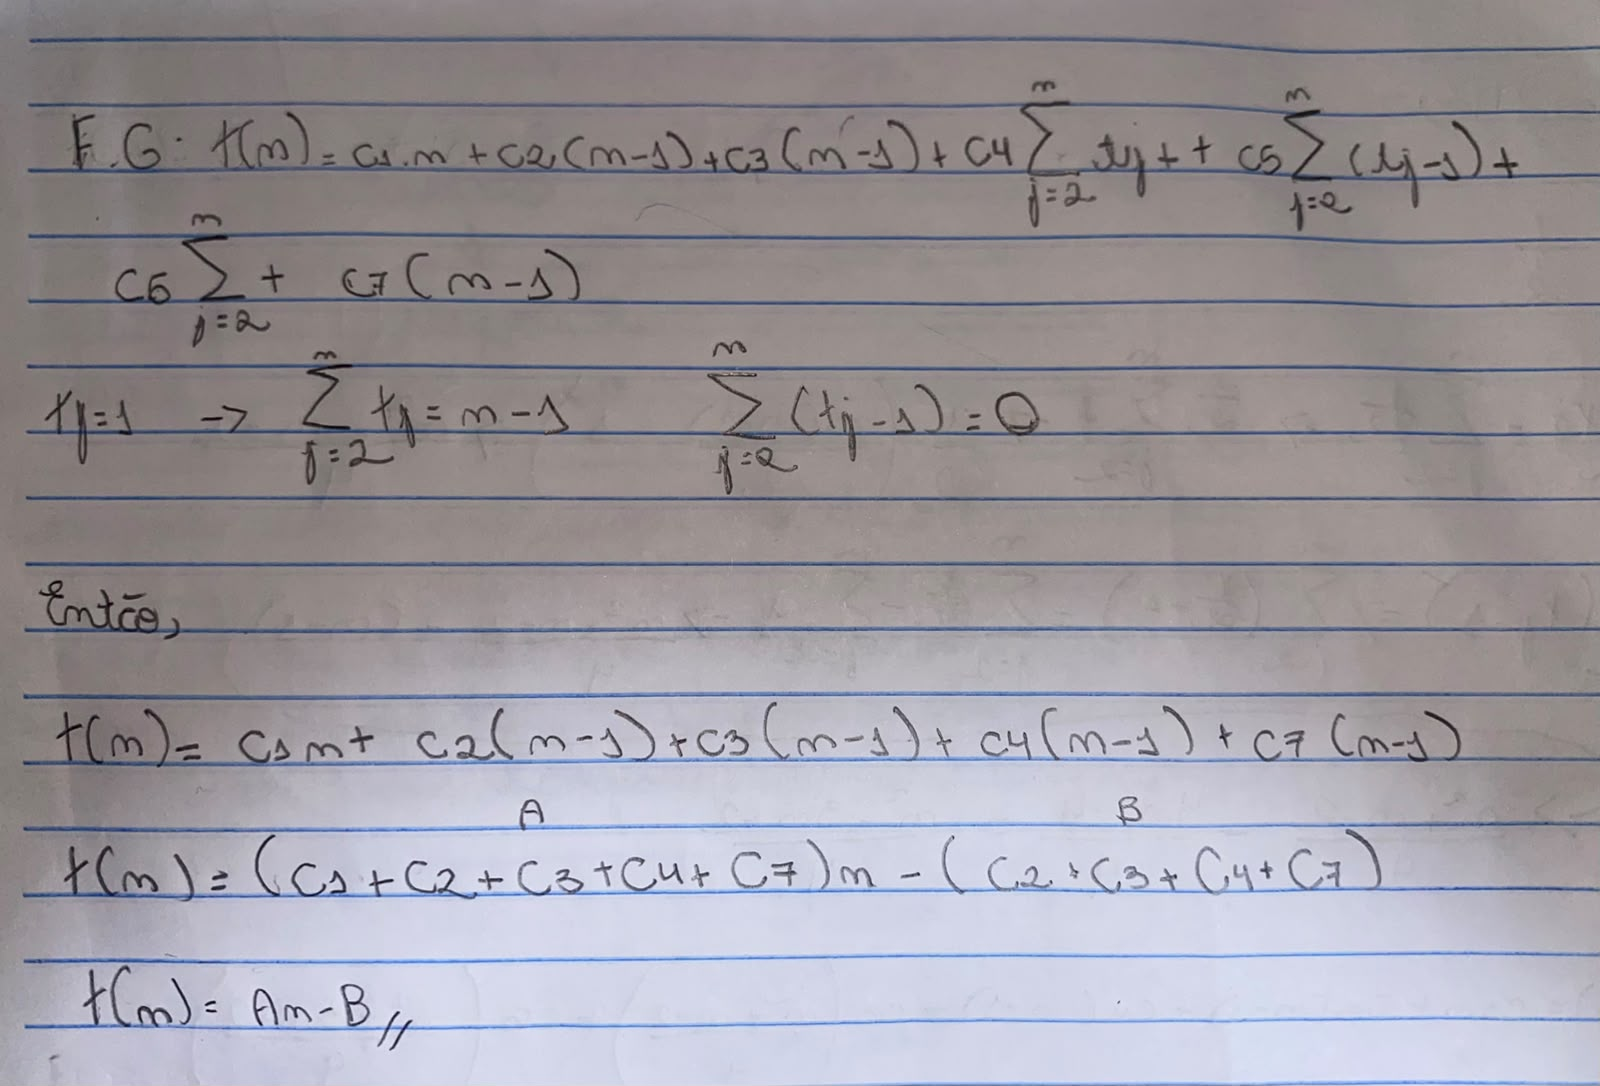
\includegraphics[width=\textwidth,height=0.62\textheight,keepaspectratio]{Imagens/Insertion Sort/melhor_caso.jpg}
	\caption{Análise do melhor caso do Insertion Sort.}
	\label{fig:melhor_caso}
\end{figure}

\subsubsection{Caso médio}

\indent \qquad No caso médio, a entrada é aleatória e cada elemento precisa
atravessar, em média, metade do trecho já ordenado. O laço interno executa
cerca de $n^2/4$ vezes, e o custo é quadrático, $O(n^2)$. A dedução está na
Figura \ref{fig:caso_medio}.

\begin{figure}[H]
	\centering
	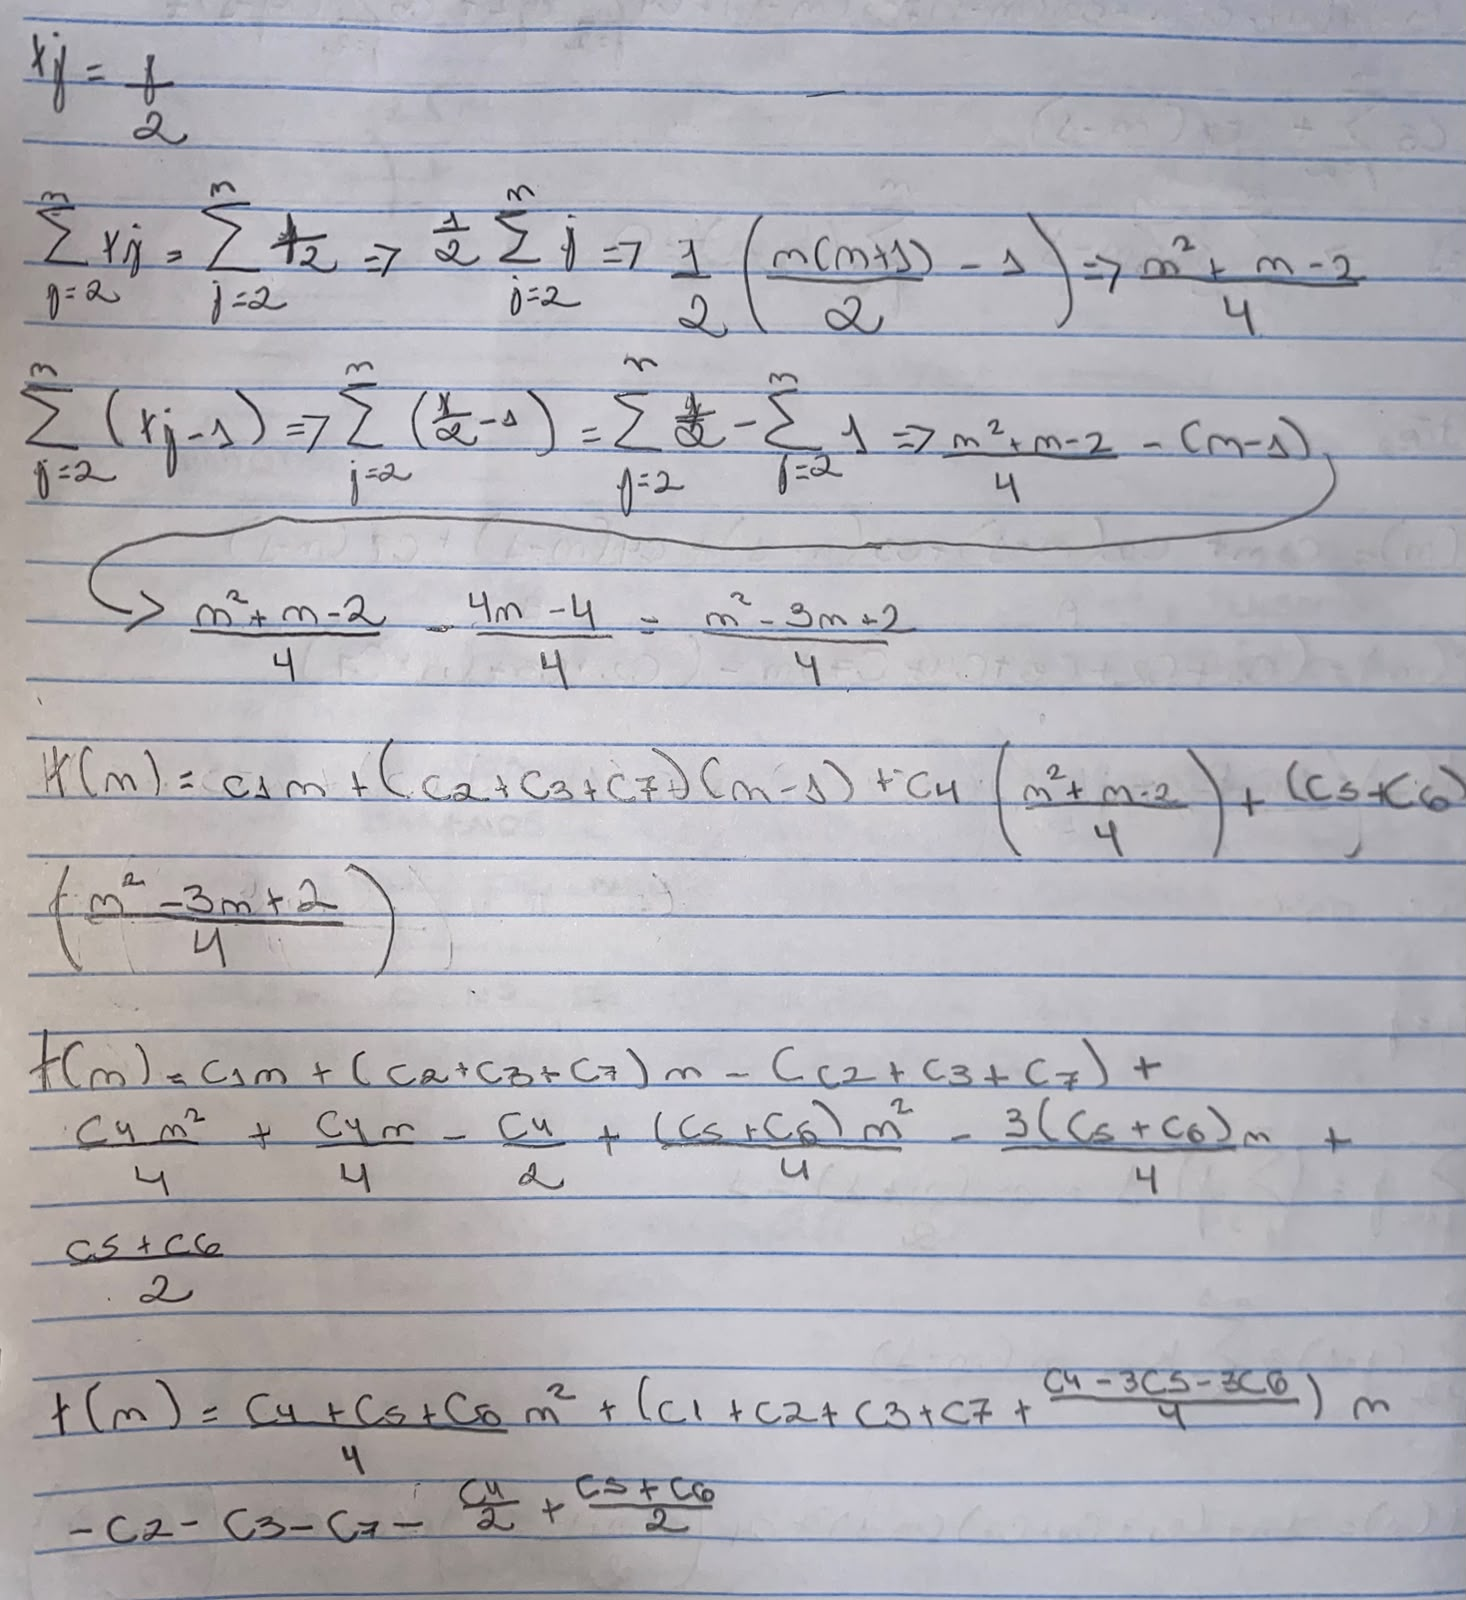
\includegraphics[width=\textwidth,height=0.62\textheight,keepaspectratio]{Imagens/Insertion Sort/caso_medio.jpg}
	\caption{Análise do caso médio do Insertion Sort.}
	\label{fig:caso_medio}
\end{figure}

\subsubsection{Pior caso}

\indent \qquad O pior caso ocorre quando o vetor está em ordem decrescente.
Cada elemento é menor que todos os anteriores e atravessa o trecho ordenado
inteiro: o laço interno executa cerca de $n^2/2$ vezes, o dobro do caso médio.
O custo é quadrático, $O(n^2)$. A dedução está na Figura \ref{fig:pior_caso}.

\begin{figure}[H]
	\centering
	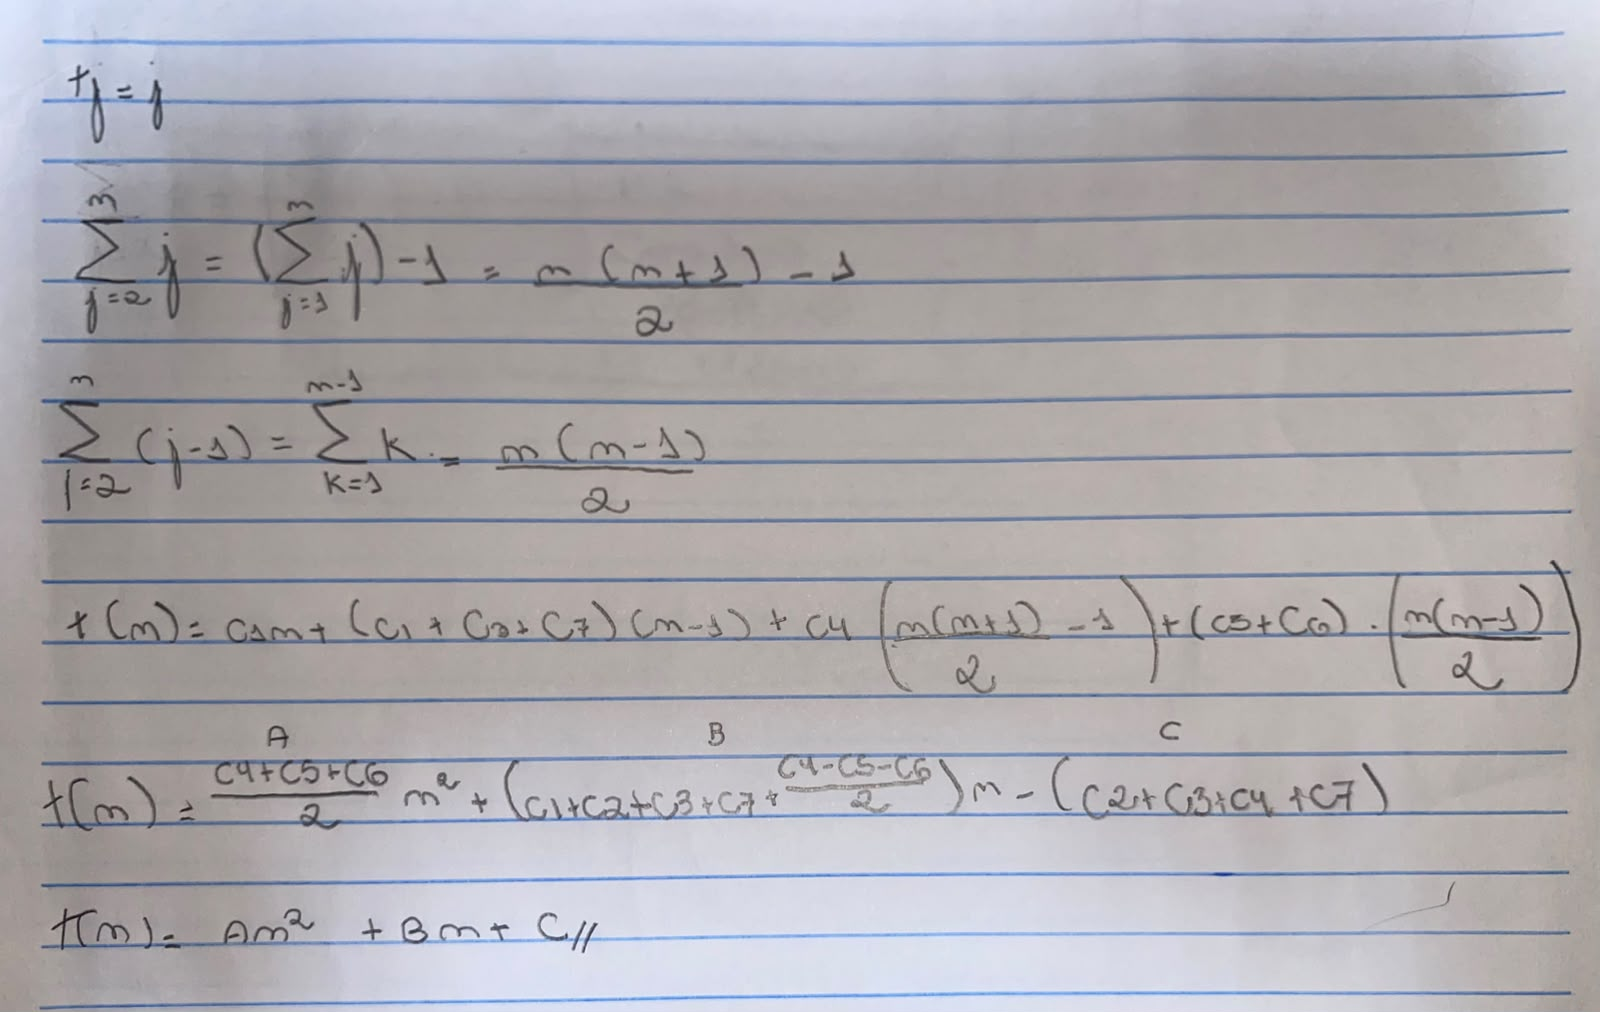
\includegraphics[width=\textwidth,height=0.62\textheight,keepaspectratio]{Imagens/Insertion Sort/pior_caso.jpg}
	\caption{Análise do pior caso do Insertion Sort.}
	\label{fig:pior_caso}
\end{figure}
